\input ../SlidePreamble
\input ../preamble

\begin{document}

{\Huge
  \centerline{\bf TTIC 31230,  Fundamentals of Deep Learning}
  \vfill
  \centerline{David McAllester, Winter 2019}
  \vfill
  \centerline{\bf The History of Deep Learning}
  \vfill
  \centerline{\bf  and Moore's Law of AI}

\vfill
\vfill

\slide{Early History}

{\bf 1943}: McCullock and Pitts introduced the linear threshold ``neuron''.

\vfill
{\bf 1962}: Rosenblatt applies a ``Hebbian'' learning rule.  Novikoff proved the perceptron convergence theorem.

\vfill
{\bf 1969}: Minsky and Papert publish the book {\it Perceptrons}.

\vfill
The Perceptrons book greatly discourages work in artificial neural networks.  Symbolic methods dominate AI research through the 1970s.

\slide{80s Renaissance}

{\bf 1980}: Fukushima introduces the neocognitron (a form of CNN)

\vfill
{\bf 1984}: Valiant defines PAC learnability and stimulates learning theory. Wins the Turing Award in 2010.

\vfill
{\bf 1985}: Hinton and Sejnowski introduce the Boltzman machine

\vfill
{\bf 1986}: Rummelhart, Hinton and Williams demonstrate empirical success with backpropagation (itself dating back to 1961).

\slide{90s and 00s: Research In the Shadows}

{\bf 1997}: Schmidhuber et al. introduce LSTMs

\vfill
{\bf 1998}: LeCunn introduces convolutional neural networks (CNNs) (LeNet).

\vfill
{\bf 2003}: Bengio introduces neural language modeling.

\slide{Current Era}

{\bf 2012}: Alexnet dominates the Imagenet computer vision challenge.

\vfill
Google speech recognition converts to deep learning.

\vfill
Both developments come out of Hinton's group in Toronto.

\vfill
{\bf 2013}: Refinement of AlexNet continues to dramatically improve computer vision.

\slide{Current Era}

{\bf 2014}: Neural machine translation appears (Seq2Seq models).

\vfill
Variational auto-encoders (VAEs) appear.

\vfill
Generative Adversarial Networks (GANs) appear.

\vfill
Graph neural networks appear (GNNs) revolutionizing the prediction of molecular properties.

\vfill
Dramatic improvement in computer vision and speech recognition continues.

\slide{Current Era}

{\bf 2015}: Google converts to neural machine translation leading to dramatic improvements.

\vfill
ResNet (residual connections) appear.  This makes yet another dramatic improvement in computer vision.

\vfill
{\bf 2016}: Alphago defeats Lee Sedol.

\slide{Current Era}

{\bf 2017}: AlphaZero learns both go and chess at super-human levels in a mater of hours entirely form self-play and advances computer go far beyond human abilities.

\vfill
Unsupervised machine translation is demonstrated.

\vfill
Progressive GANs demonstrate high resolution realistic face generation.

\slide{Current Era}

{\bf 2018}: Unsupervised pre-training significantly improves a broad range of NLP tasks including question answering (but dialogue remains unsolved).

\vfill
AlphaFold revolutionizes protein structure prediction.

\vfill{\bf 2019}:
Vector quantized VAEs (VQ-VAE) demstrate that VAEs can be competative with GANs for high-resolution image generation.

\vfill
Super-human performance is achieved on the GLUE natural langauge understanding benchmark.

\slide{2019: Natural Language Understanding}

GLUE: General Language Understanding Evaluation

\vfill

\centerline{\normalsize ArXiv 1804.07461}
\centerline{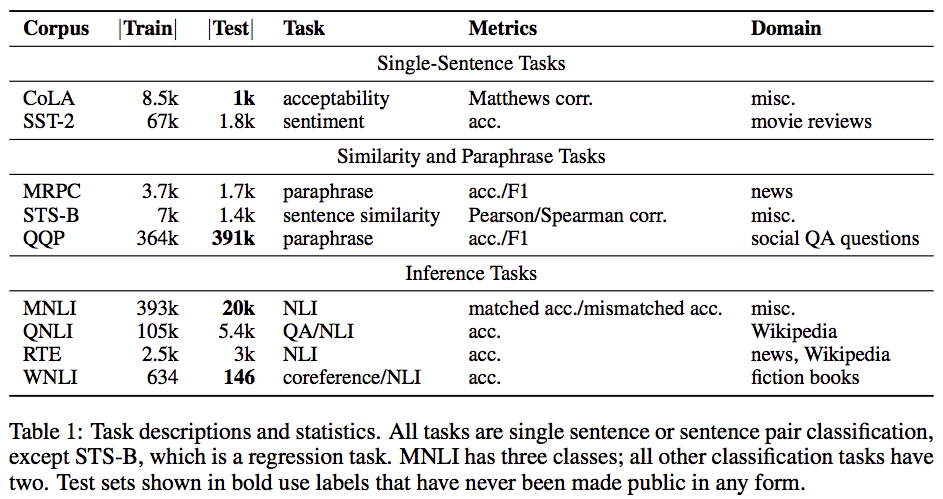
\includegraphics[width= 7in]{\images/GLUE}}

\slide{BERT and GLUE}

\centerline{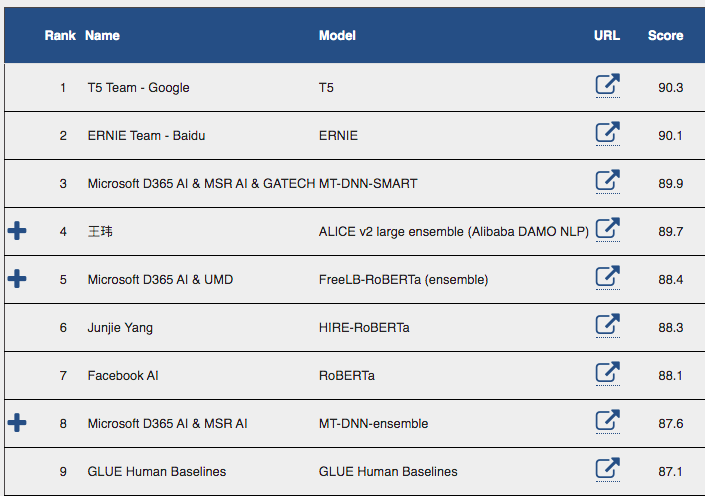
\includegraphics[width= 7in]{\images/GLUELeader}}

\slide{BERT and SuperGLUE}

\centerline{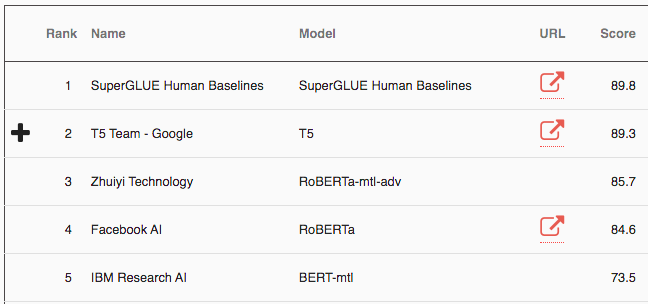
\includegraphics[width= 9in]{\images/SuperLeader}}

\slidetwo{Generative Adversarial Nets (GANs)}{Goodfellow et al., 2014}
\centerline{\includegraphics[width = 9in]{/users/davidmcallester/tex/images/GAN2014}}


\slide{Moore's Law of AI}
\centerline{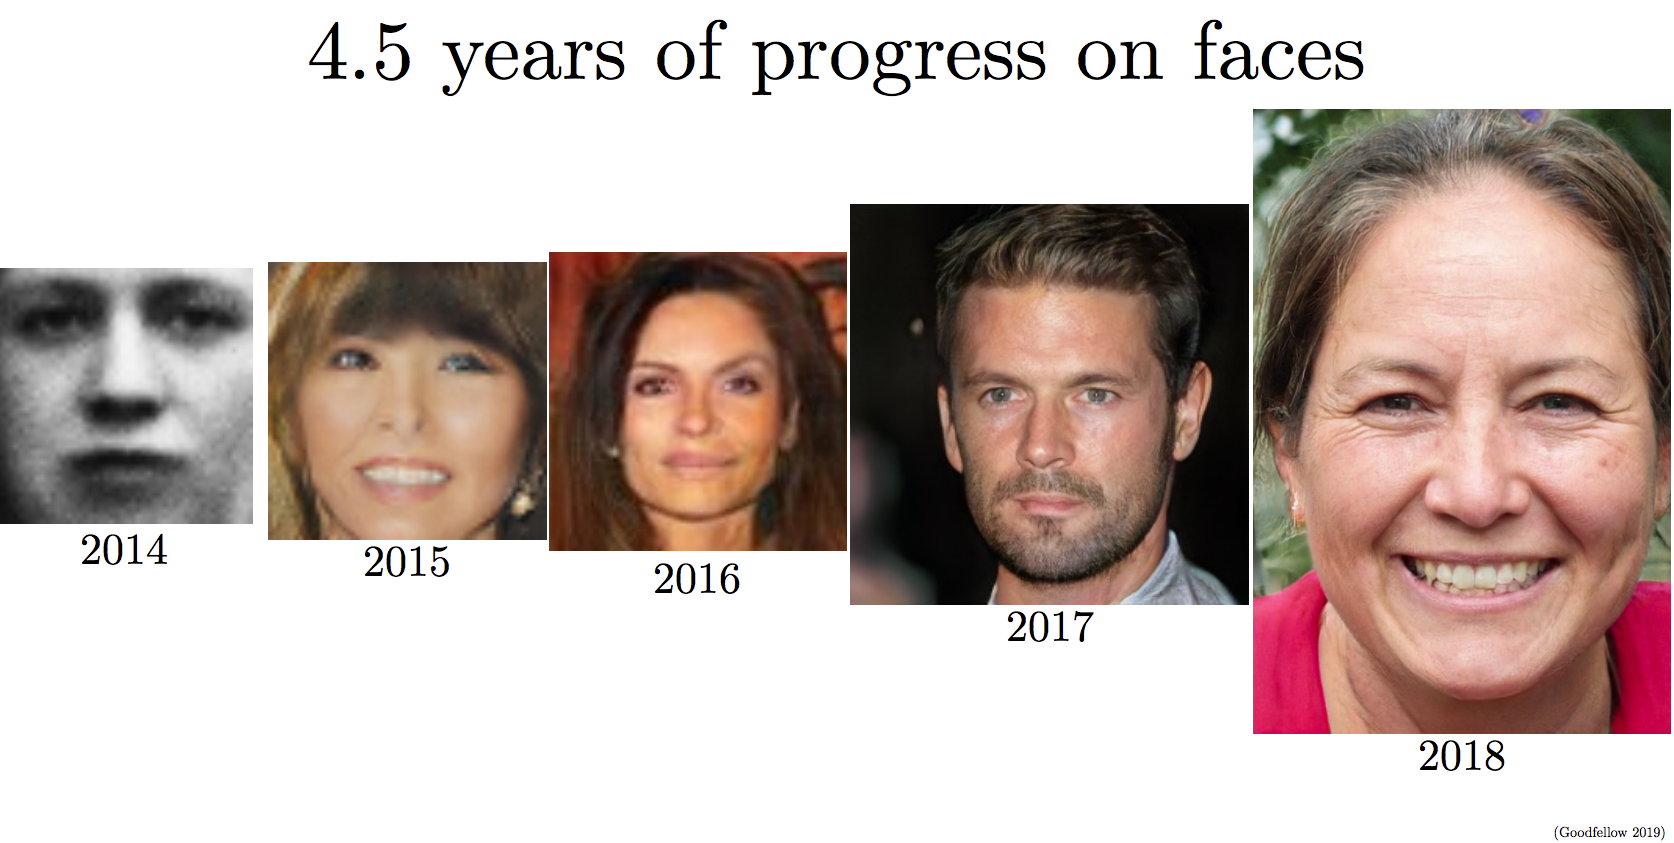
\includegraphics[height = 4.5in]{\images/GoodfellowInvited1}}

ArXiv 1406.2661, 1511.06434, 1607.07536, 1710.10196, 1812.04948

\centerline{Goodfellow, ICLR 2019 Invited Talk}

\slide{GANs for Imagenet}

\centerline{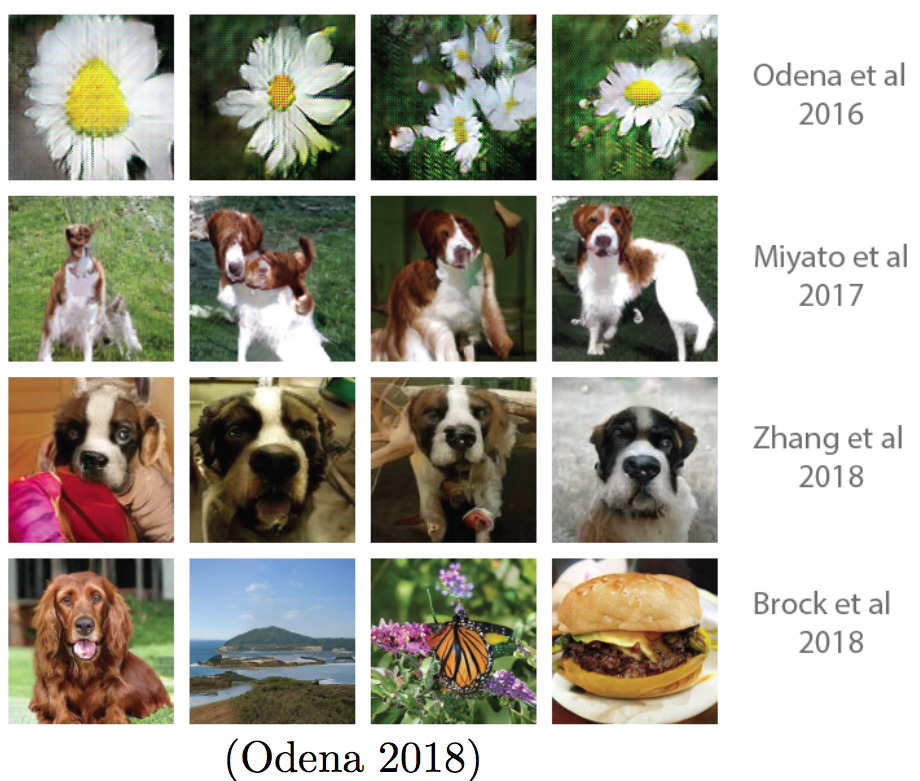
\includegraphics[height = 5.0in]{\images/GoodfellowInvited2}}

\slide{BigGANs, Brock et al., 2018}

\centerline{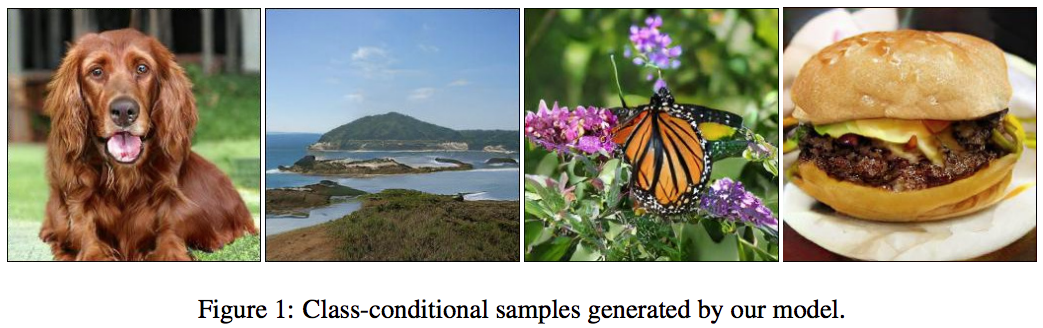
\includegraphics[width = 10.0in]{\images/BigGANs}}

\slide{Variational Auto Encoders (VAEs, 2015)}

\centerline{\includegraphics[width = 4in]{/users/davidmcallester/tex/images/VariationalFaces}}
\centerline{[Alec Radford, 2015]}

\slide{VAEs in 2019}

\centerline{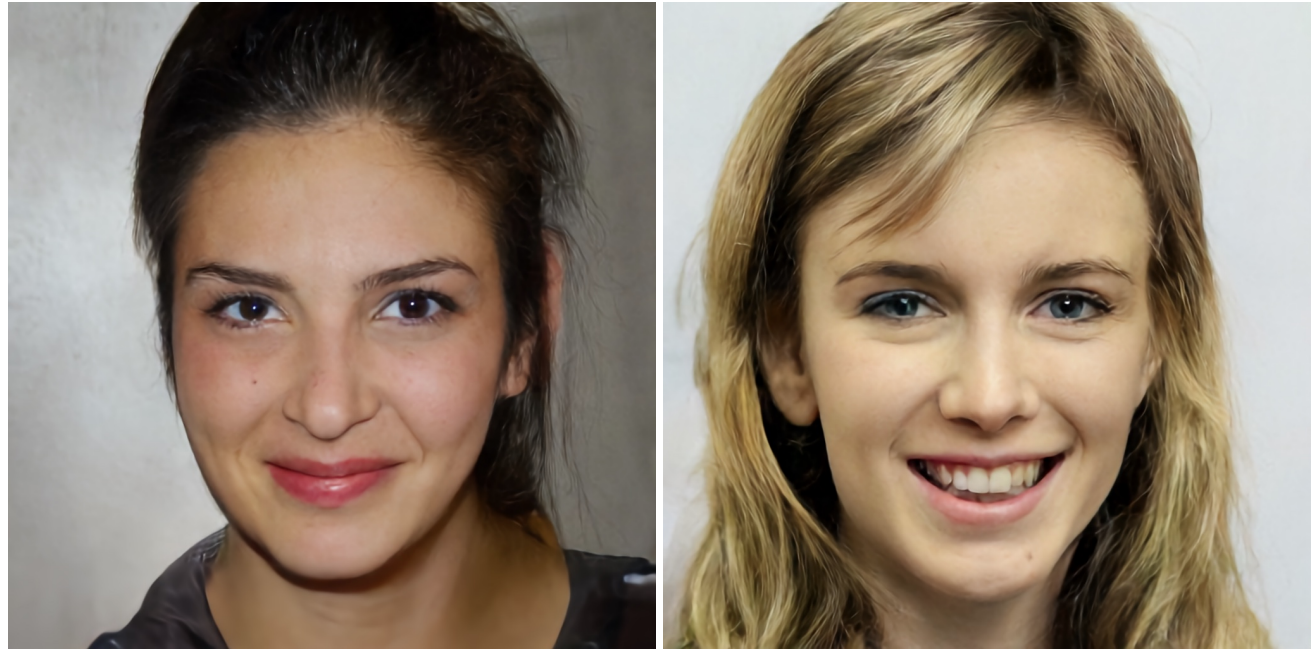
\includegraphics[width = 8in]{\images/VQ-VAE22}}

\vfill
VQ-VAE-2, Razavi et al. June, 2019

\slide{VAEs in 2019}

\centerline{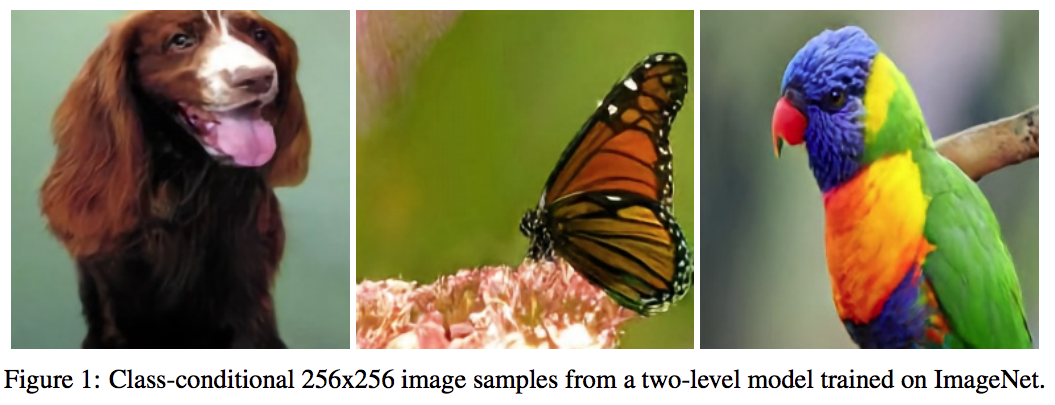
\includegraphics[width = 10in]{/users/davidmcallester/tex/images/VQ-VAE21}}

\vfill
VQ-VAE-2, Razavi et al. June, 2019

\slideplain{END}

}
\end{document}
